\documentclass[11pt]{article}
\usepackage{amsmath,amsthm,amssymb,fullpage,graphicx,hyperref,listings}
\usepackage{listings,color,setspace}
\author{Andy Reagan}
\title{Math 337 Homework 15}

     \def\NN{\mathbb{N} }
     \def\ZZ{\mathbb{Z} }
     \def\QQ{\mathbb{Q} }
     \def\RR{\mathbb{R} }
     \def\CC{\mathbb{C} }
     \def\f{\frac }
     \def\b{\begin }
     \def\e{\end }
     \def\Log{\text{Log} \,}
     \def\Re{\text{Re} \, }
     \newcommand{\pdiff}[2]{\frac{\partial #1}{\partial #2}}
     \newcommand{\partialdiff}[2]{\frac{\partial #1}{\partial #2}}
     \newcommand{\pdiffsq}[2]{\frac{\partial^2 #1}{{\partial #2}^2}}
     \newcommand{\pdiffcu}[2]{\frac{\partial^3 #1}{{\partial #2}^3}}
     \newcommand{\pdiffhi}[3]{\frac{\partial^#3 #1}{{\partial #2}^#3}}
     \newcommand{\diff}[2]{\frac{{\rm d}#1}{{\rm d}#2}}
     \newcommand{\diffsq}[2]{\frac{{\rm d}^{2}#1}{{\rm d} {#2}^2}}
     \newcommand{\diffhi}[3]{\frac{{\rm d}^#3 #1}{{\rm d} {#2}^#3}}
     \newcommand{\tdiff}[2]{\mbox{d} #1/\mbox{d} #2}
     \newcommand{\tdiffsq}[2]{\mbox{d}^{2} #1/\mbox{d} {#2}^2}
     \newcommand{\tpdiff}[2]{\partial #1/\partial #2}
     \newcommand{\tpdiffsq}[2]{\partial^2 #1/\partial {#2}^2}
     \newcommand{\bvec}[1]{\vec{ {\bf #1 } }}
     \newcommand{\oh}[1]{O(h^{{#1}})}

\lstset{language=MATLAB,
basicstyle=\ttfamily\scriptsize\singlespacing,
keywordstyle=\color{black},
stringstyle=\color{black},
commentstyle=\color{black},
morecomment=[l][\color{black}]{\#},
frame=L,
xleftmargin=\parindent,
%%numbers=left,                   %% where to put the line-numbers
%%numberstyle=\scriptsize,      %% the size of the fonts that are used for the line-numbers
%%stepnumber=1,                   %% the step between two line-numbers. If it is 1 each line will be numbered
numbersep=5pt,
breaklines=true,        %% sets automatic line breaking
breakatwhitespace=false,    %% sets if automatic breaks should only happen at whitespace
escapeinside={\%*}{*)} 
}

%% example code insert
%% \lstinputlisting[language=Matlab]{andy_hw12_prb01.m}

%% example figure
%% \begin{figure}[h!]
%%   \centering
%%     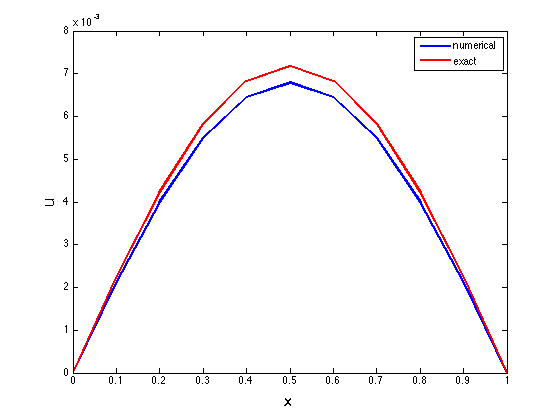
\includegraphics[width=0.45\textwidth]{andy_hw12_prb01_02.png}
%%   \caption{The numerical and exact solution for $h=0.1$.}
%% \end{figure}

%% start problem on next page
%% \clearpage
%% \pagebreak

\begin{document}
\maketitle

\begin{enumerate}

\item Done.

\item Done.

\item First we'll rewrite the half angle formula into a form more useful directly (starting the form given above Eq 12.35 in the notes):
\begin{align*} & 1-\cos \alpha = 2 \sin ^2 \left ( \f{\alpha}{2} \right ) \\
&2-2\cos \alpha = 4 \sin ^2 \left ( \f{\alpha}{2} \right ) \\
&2\cos \alpha - 2= - 4 \sin ^2 \left ( \f{\alpha}{2} \right ) \end{align*}
Now, we'll show Eq 15.12 directly.
\begin{align*} \delta _x ^2 \left [ e^{i\beta m h} e^{i\gamma l h} \right ] &= e^{i\beta (m+1) h} e^{i\gamma l h} -2 e^{i\beta m h} e^{i\gamma l h} + e^{i\beta (m-1) h} e^{i\gamma l h}\\
&= e^{i\beta m h} e^{i\gamma l h} \left [ e^{i\beta h}-2  + e^{-i\beta h} \right ]\\
&= e^{i\beta m h} e^{i\gamma l h} \left [ 2\cos (\beta h) -2 \right ]\\
&= e^{i\beta m h} e^{i\gamma l h} \left [ -4 \sin ^2 \left ( \f{\beta h}{2} \right ) \right ]\\
&= -4 \sin ^2 \left ( \f{\beta h}{2} \right )  \left [ e^{i\beta m h} e^{i\gamma l h}\right ]\end{align*}
We now do the same for Eq 15.13:
\begin{align*} \delta _y ^2 \left [ e^{i\beta m h} e^{i\gamma l h} \right ] &= e^{i\beta m h} e^{i\gamma (l+1) h} -2 e^{i\beta m h} e^{i\gamma l h} + e^{i\beta m h} e^{i\gamma (l-1) h}\\
&= e^{i\beta m h} e^{i\gamma l h} \left [ e^{i\gamma h}-2  + e^{-i\gamma h} \right ]\\
&= e^{i\beta m h} e^{i\gamma l h} \left [ 2\cos (\gamma h) -2 \right ]\\
&= e^{i\beta m h} e^{i\gamma l h} \left [ -4 \sin ^2 \left ( \f{\gamma h}{2} \right ) \right ]\\
&= -4 \sin ^2 \left ( \f{\gamma h}{2} \right )  \left [ e^{i\beta m h} e^{i\gamma l h}\right ]\end{align*}

% 4
\item

% 5
\item

% 6
\item First I make note of the very important considerations mentioned in the paragraph following Eq 15.37, which make clear the notation that we are using.
Namely, we are solving for a solution in a 2D space (with solution represented as a matrix), where discretizations have been made in orthogonal directions.
We choose to break this into a smaller problems: we solve not for the full solution at the next timestep, but rather we solve for each column, one at a time.
In doing so, we first break the problem in columns, which in turn determines which operators act as matrices on a columns, and which operate across columns.
We have chosen to break into columns where $m$ varies, namely columns for each $l$.
Doing this, we arrive at Eq 15.37.
To make this more clear, consider Eq 15.37 in matrix form:
\begin{align*} & \left [ \left ( \begin{array}{ccc} 1 & 0 & 0\\ 0 & 1 & 0\\ 0 & 0 & 1 \end{array} \right )  - \f{r}{2} \left ( \begin{array}{ccc} -2 & 1 & 0\\ 1 & -2 & 1\\ 0 & 1 & -2 \end{array} \right )\right ] \left ( \begin{array}{c} U_{1,l} \\ U_{2,l} \\ U_{3,l} \end{array} \right ) ^{*} = \left ( \begin{array}{c} U_{1,l} \\ U_{2,l} \\ U_{3,l} \end{array} \right ) ^{n} \\
&~~~~~~~~~~~~~~~+ \f{r}{2} \left [ \left ( \begin{array}{c} U_{1,l+1} \\ U_{2,l+1} \\ U_{3,l+1} \end{array} \right ) ^{n} - 2\left ( \begin{array}{c} U_{1,l} \\ U_{2,l} \\ U_{3,l} \end{array} \right ) ^{n} + \left ( \begin{array}{c} U_{1,l-1} \\ U_{2,l-1} \\ U_{3,l-1} \end{array} \right ) ^{n}\right ] \end{align*}
Since $L = 5$, we solve for $U^{*}$ for $l = 1\cdot 4$, where the BC of $U^{*}$ at $l = 0, 5$ are given by the prescribed conditions.
Here, they are just 0.
We observe that for $l=1$ and $l=4$ the RHS $U^{n}$ will have $l=0,5$ respectively, where here we invoke the BC.
So what we are really solving for is a $(M-2) \times (L-2)$ matrix from a $M\times L$ matrix, solving for only the inner points.

We could write out the previous equation for each $L$, but this is cumbersome and is not how we will solve the problem on a computer.
Namely, we will solve this as a matrix, for all of the columns.
Without further adieu, this is:
\begin{align*} & \left [ \left ( \begin{array}{ccc} 1 & 0 & 0\\ 0 & 1 & 0\\ 0 & 0 & 1 \end{array} \right )  - \f{r}{2} \left ( \begin{array}{ccc} -2 & 1 & 0\\ 1 & -2 & 1\\ 0 & 1 & -2 \end{array} \right )\right ] \left ( \begin{array}{cccc} U_{1,1} & U_{1,2} & U_{1,3} & U_{1,4 }\\ U_{2,1} & U_{2,2} & U_{2,3} & U_{2,4 } \\ U_{3,1} & U_{3,2} & U_{3,3} & U_{3,4 }  \end{array} \right ) ^{*} \\
& ~~~~~~~~~= \left ( \begin{array}{cccc} U_{1,1} & U_{1,2} & U_{1,3} & U_{1,4 }\\ U_{2,1} & U_{2,2} & U_{2,3} & U_{2,4 } \\ U_{3,1} & U_{3,2} & U_{3,3} & U_{3,4 }  \end{array} \right ) ^{n} + \f{r}{2} \left [ \left ( \begin{array}{cccc} U_{1,2} & U_{1,3} & U_{1,4} & 0 \\ U_{2,2} & U_{2,3} & U_{2,4} & 0 \\ U_{3,2} & U_{3,2} & U_{3,4} & 0  \end{array} \right ) ^{n} \right.\\
& ~~~~~~~~~\left. -2\left ( \begin{array}{cccc} U_{1,1} & U_{1,2} & U_{1,3} & U_{1,4 }\\ U_{2,1} & U_{2,2} & U_{2,3} & U_{2,4 } \\ U_{3,1} & U_{3,2} & U_{3,3} & U_{3,4 }  \end{array} \right ) ^{n} + \left ( \begin{array}{cccc} 0 & U_{1,1} & U_{1,2} & U_{1,3 }\\ 0 & U_{2,1} & U_{2,2} & U_{2,3 } \\ 0 & U_{3,1} & U_{3,2} & U_{3,3 }  \end{array} \right ) ^{n} \right ]\end{align*}

Regardless about solving on the computer, from the above is obvious how the problem is split into columns.
If it is not, just take the first column from every $3\times 4$ matrix for the first column problem, the second column from every $3\times 4$ matrix for the second column problem, and so forth.
The boundary conditions have entered visibly only in $l$ since they are zero.
If they were nonzero along $x=0$ or $x=M$ the $3\times 3$ matrix on the LHS (resulting from the addition) would need a $\bvec{b}$ vector on the LHS when solving for each column, added outside what is already there, with the nonzero boundary conditions included at the beginning and end of this vector as we have done in the past.
In the matrix form above, this would actually be a matrix, $\bvec{B}$.

Next, we write Eq 15.34(b) 
\begin{align*} & \left [ \left ( \begin{array}{cccc} 1 & 0 & 0 & 0\\ 0 & 1 & 0 & 0\\ 0 & 0 & 1 & 0\\ 0 & 0 & 0 & 1\end{array} \right )  - \f{r}{2} \left ( \begin{array}{cccc} -2 & 1 & 0 & 0 \\ 1 & -2 & 1 & 0\\ 0 & 1 & -2 & 1\\ 0 & 0 & 1 & -2\end{array} \right )\right ] \left ( \left ( \begin{array}{cccc} U_{1,1} & U_{1,2} & U_{1,3} & U_{1,4 }\\ U_{2,1} & U_{2,2} & U_{2,3} & U_{2,4 } \\ U_{3,1} & U_{3,2} & U_{3,3} & U_{3,4 }  \end{array} \right ) ^T \right ) ^{n+1} \\
& ~~~~~~~~~= \left ( \left ( \begin{array}{cccc} U_{1,1} & U_{1,2} & U_{1,3} & U_{1,4 }\\ U_{2,1} & U_{2,2} & U_{2,3} & U_{2,4 } \\ U_{3,1} & U_{3,2} & U_{3,3} & U_{3,4 }  \end{array} \right )  ^T \right )  ^{*} + \f{r}{2} \left [ \left ( \left ( \begin{array}{cccc} U_{1,2} & U_{1,3} & U_{1,4} & 0 \\ U_{2,2} & U_{2,3} & U_{2,4} & 0 \\ U_{3,2} & U_{3,2} & U_{3,4} & 0  \end{array} \right ) ^T \right ) ^{*} \right.\\
& ~~~~~~~~~\left. -2\left ( \left ( \begin{array}{cccc} U_{1,1} & U_{1,2} & U_{1,3} & U_{1,4 }\\ U_{2,1} & U_{2,2} & U_{2,3} & U_{2,4 } \\ U_{3,1} & U_{3,2} & U_{3,3} & U_{3,4 }  \end{array} \right ) ^T \right ) ^{*} + \left ( \left ( \begin{array}{cccc} 0 & U_{1,1} & U_{1,2} & U_{1,3 }\\ 0 & U_{2,1} & U_{2,2} & U_{2,3 } \\ 0 & U_{3,1} & U_{3,2} & U_{3,3 }  \end{array} \right ) ^T \right ) ^{*} \right ]\end{align*}

where again we can solve this equation column by column for the three columns of $U^{n+1}$ in matrix form above.

% 7
\item This was already discussed in problem 6, in a manner in which is sufficient to code.
But I will still elaborate more.
Specifically, we first solve for $U ^*$ column by column, and the using this $U^*$, we solve for $U ^{n+1}$ column by column.

I am inclined to try solving this as a matrix eqaution, as we discussed in class, and if I try this to compare, I will report on the results.
Of course, this is only reasonable to try for the case of 0 boundary conditions, since even for Dirichlet BC the determination of the BC of the intermediate solution $U^*$ is no longer trivial.
Pre-computing $\bvec{b}^*$ could, in theory, make this possible even for nonzero BC conditions.

I'll note that I choose to update the BC for $U^{n+1}$ at the end of the time loop, since this makes the most sense to me (determing $U^{n+1}$ happens in one place).

% 8
\item I solve the problem using the method that was exhaustively elaborated upond above.

I am able to solve the problem as a matrix, and gain a huge speedup by doing so.
Namely, solving with a loop over the columns up to $t=3$:

\verb|Elapsed time is 0.291936 seconds.|

And solving with matrices:

\verb|Elapsed time is 0.047398 seconds.|

This is approximately a $6\times$ speedup, which is substantial.

% 9
\item Done.

% 10 
\item Attempt for Monday.

% 11
\item Somday.

% Bonus 1 (12)
\item

% Bonus 2 (13)
\item

\end{enumerate}
\end{document}



